
\chapter{MOTION PRIMITIVE TRANSITION:WALK AND STANCE}
\label{chap:stance}
    \graphicspath{{WalkStance/WalkStanceFigs/EPS/}{WalkStance/WalkStanceFigs/}}

This chapter focuses on the synthesizing transitional motions.



    
    




\section{Motion Primitives}
After a  heel strike, if the resulting velocity is not enough, passive walker will stop walking and rest at the double support posture.
This stable posture as shown in Figure ~\ref{fig:bipedalstance}, is another motion primitive: the stance. 

\begin{figure}[!htbp]
  \begin{center}
      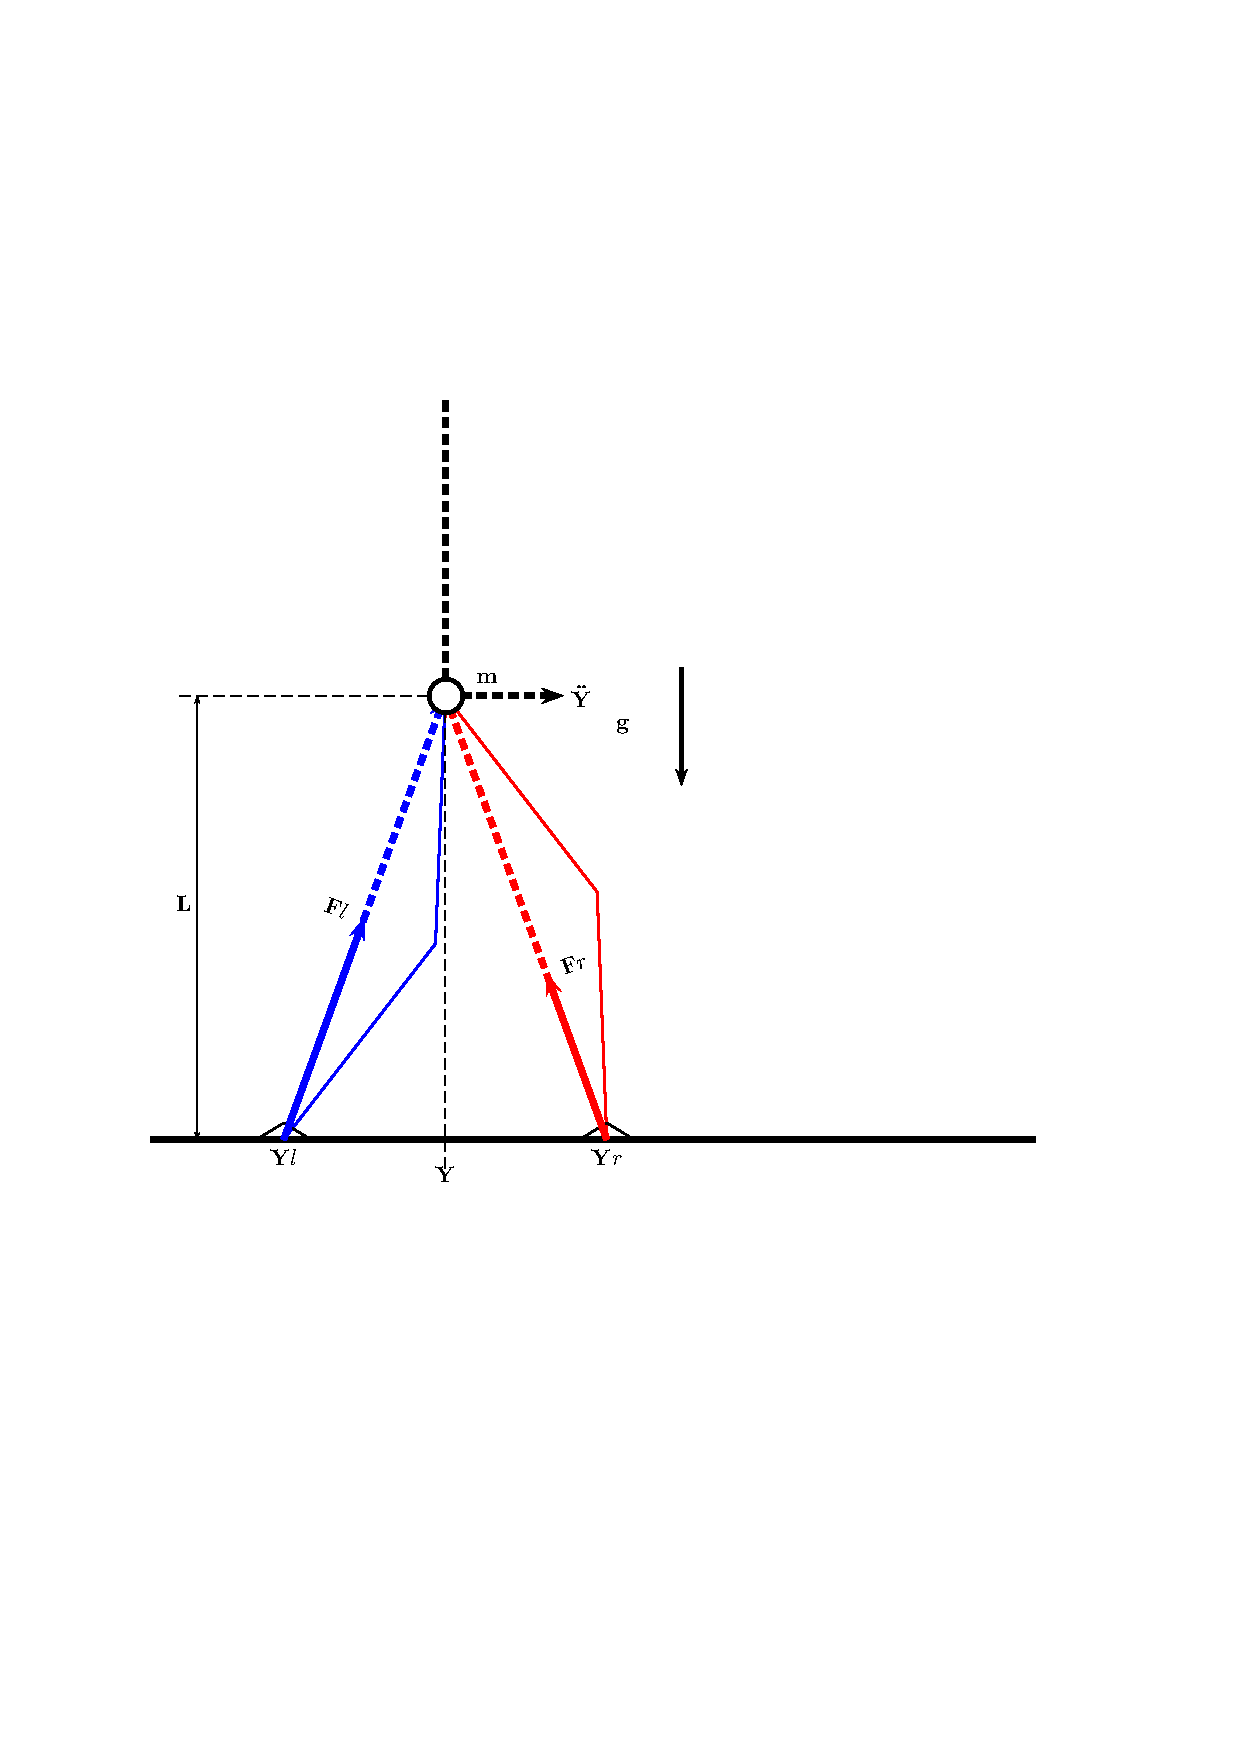
\includegraphics[width=0.7\textwidth]{stancefigure}
    \caption{The Stance Motion Primitives}
    \label{fig:bipedalstance}
\end{center}
\end{figure}


\subsection{Dynamics}
When people stand, the two legs are almost straight, 
Instead of the four link rigid body model, stance can be simplified as a point supported by two straight legs. 
\citet{stephens2009modeling} propose even the height of waist can be neglected, since is almost constant.
So dynamic model can be simplified as has one degree of freedom, the horizontal displacement.
For configurations of shank and thigh can be worked out through \emph{inverse kinematics}.
 




The dynamic is not continues, can be divided into three phases, as shown in Figure~\ref{phaseregionsofstance}

\begin{figure}[!htbp]
  \begin{center}
     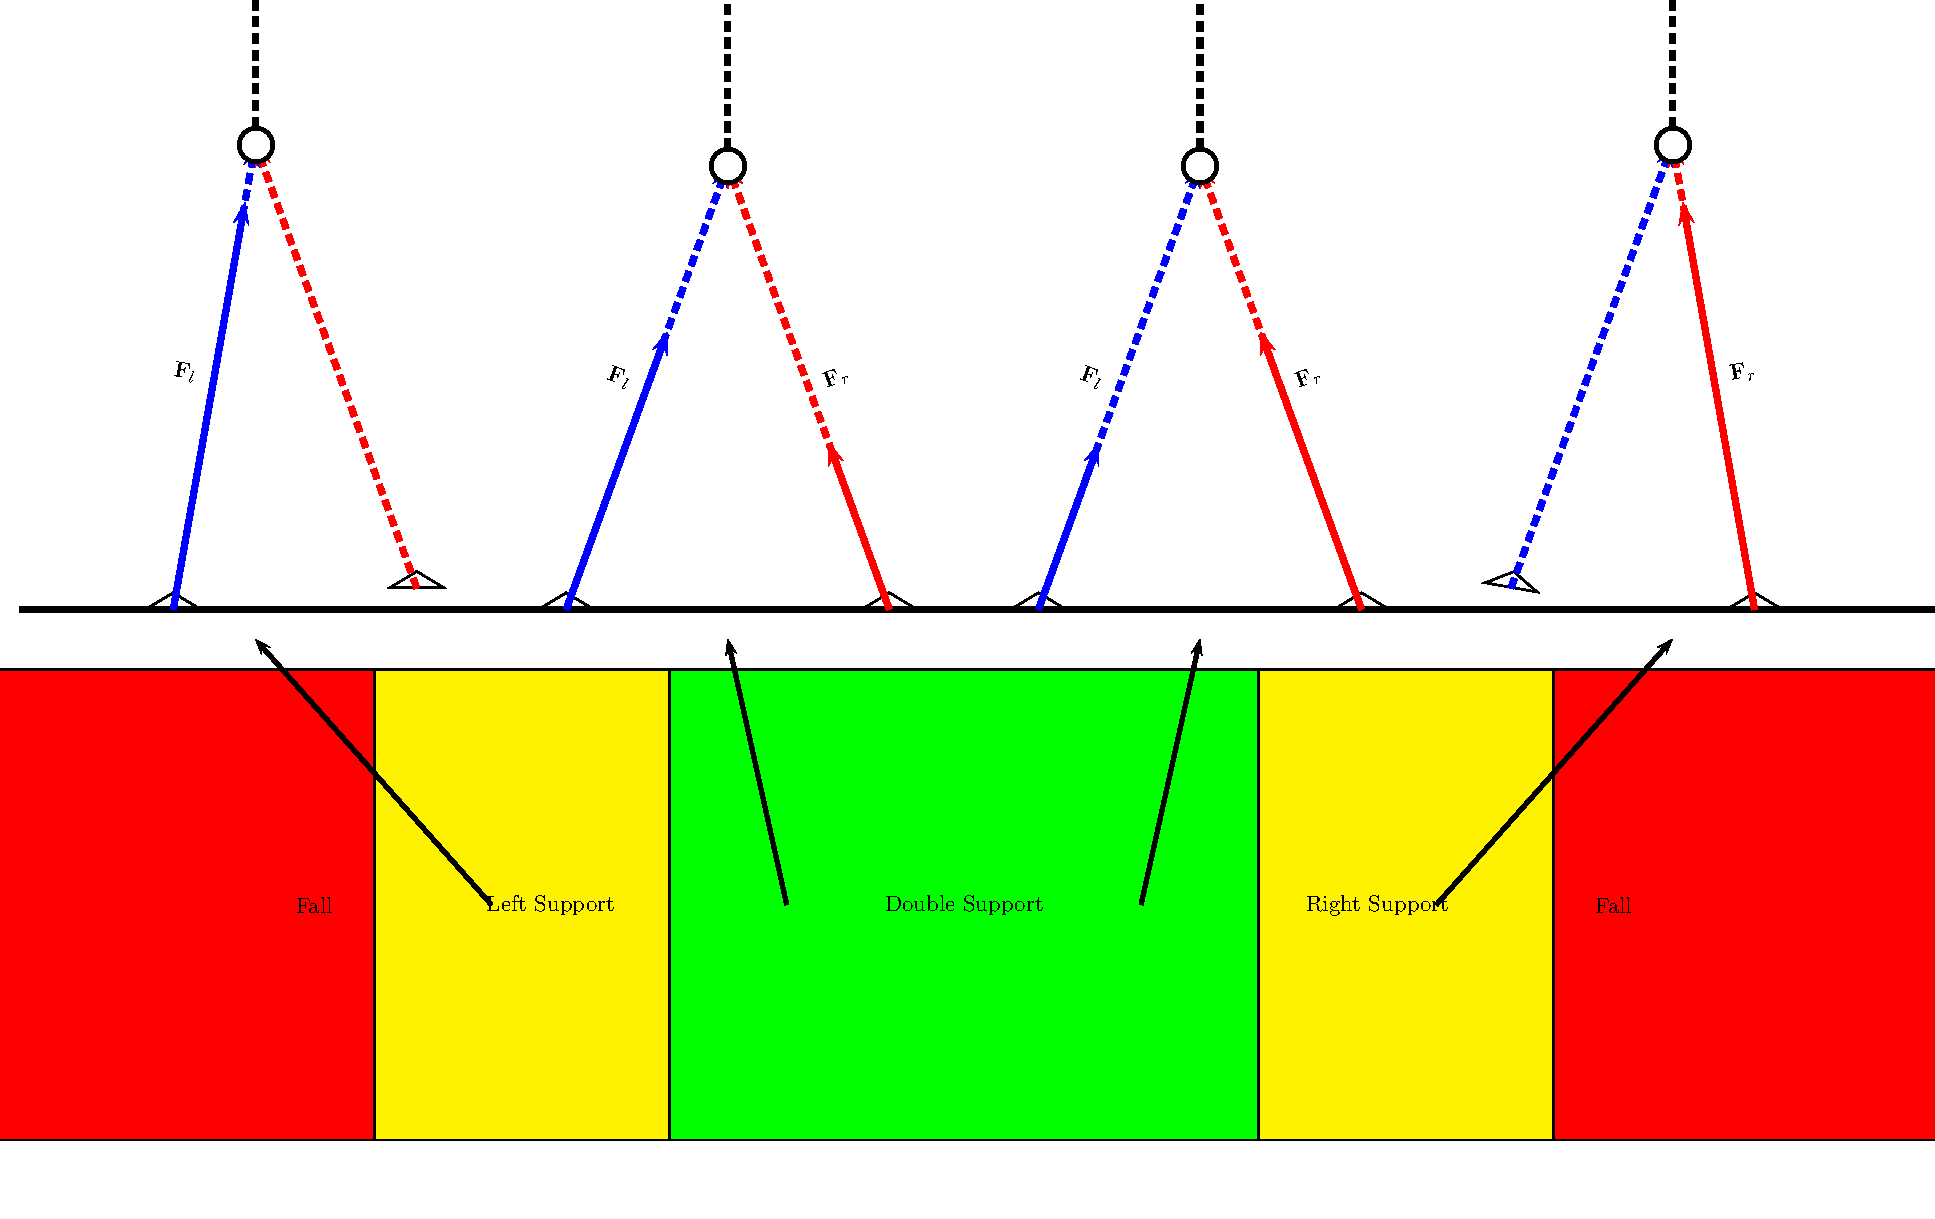
\includegraphics[width=0.7\textwidth]{stanceConfigure}
    \caption{dicontinus dynamics of stance}
    \label{fig:phaseregionsofstance}
\end{center}
\end{figure}


\begin{itemize}
\HiItem{Double Support}
When the off center  displacement  is small, people stand with two legs support.
the motion is governed by the gravity.
\[
\ddot{q}=\frac{\gv}{L}w_r(q-y_r)+\frac{gv}{L}w_l(q-y_l)
\]

Torques are generated by the two legs to maintain stability.
The torques are not be equal,intuitively,
The left torque is increased when the centre moving left, so on with the right torque.
Suppose the relationship between torques and centre position is linear.
Dynamic Equation~\ref{eq:stanceequation} incorporate the control strategy.
\begin{equation}
\label{eq:stanceequation}
\ddot{q}=\frac{\gv}{L}w_r(q-y_r)+\frac{\gv}{L}w_l(q-y_l)+\frac{\tau_L+\tau_R}{mL}
\end{equation}



\HiItem{Single Leg Support}
For a big horizontal  displacement,  people stand a single leg.
The passive dynamic is
\[
\ddot{q}=\frac{g}{L}q
\]
Equation~\ref{eq:singlestand} incorporate the torque generated by legs.
\begin{equation}
\label{eq:singlestand}
\ddot{q}=\frac{g}{L}q+\frac{y_{L,R}}{L}\tau_{L,R}
\end{equation}

\HiItem{Fall and Walk}
For even bigger displacement,  the stance posture can not be maintained.
The region where it is possible for human maintain the stand posture is called ``support region''
For a human, the width of the ``support region'' depends on the  height and the step size.
When move out the ``support region'', stance motion can't be maintained, human can either walk or fall.
\end{itemize}


Maintaining stance is to maintain the horizontal displacement within the support region.

\section {Motor Invariant Control}
\subsection{Entraintment}
Without damping effects, the original system is similar to mass spring system.
It will vibrate endlessly, as shown in Figure~\ref{fig:stancepostures}
If the speed is high, then the state will move out of the basin of attraction.

\begin{figure}[!htbp]
  \begin{center}
     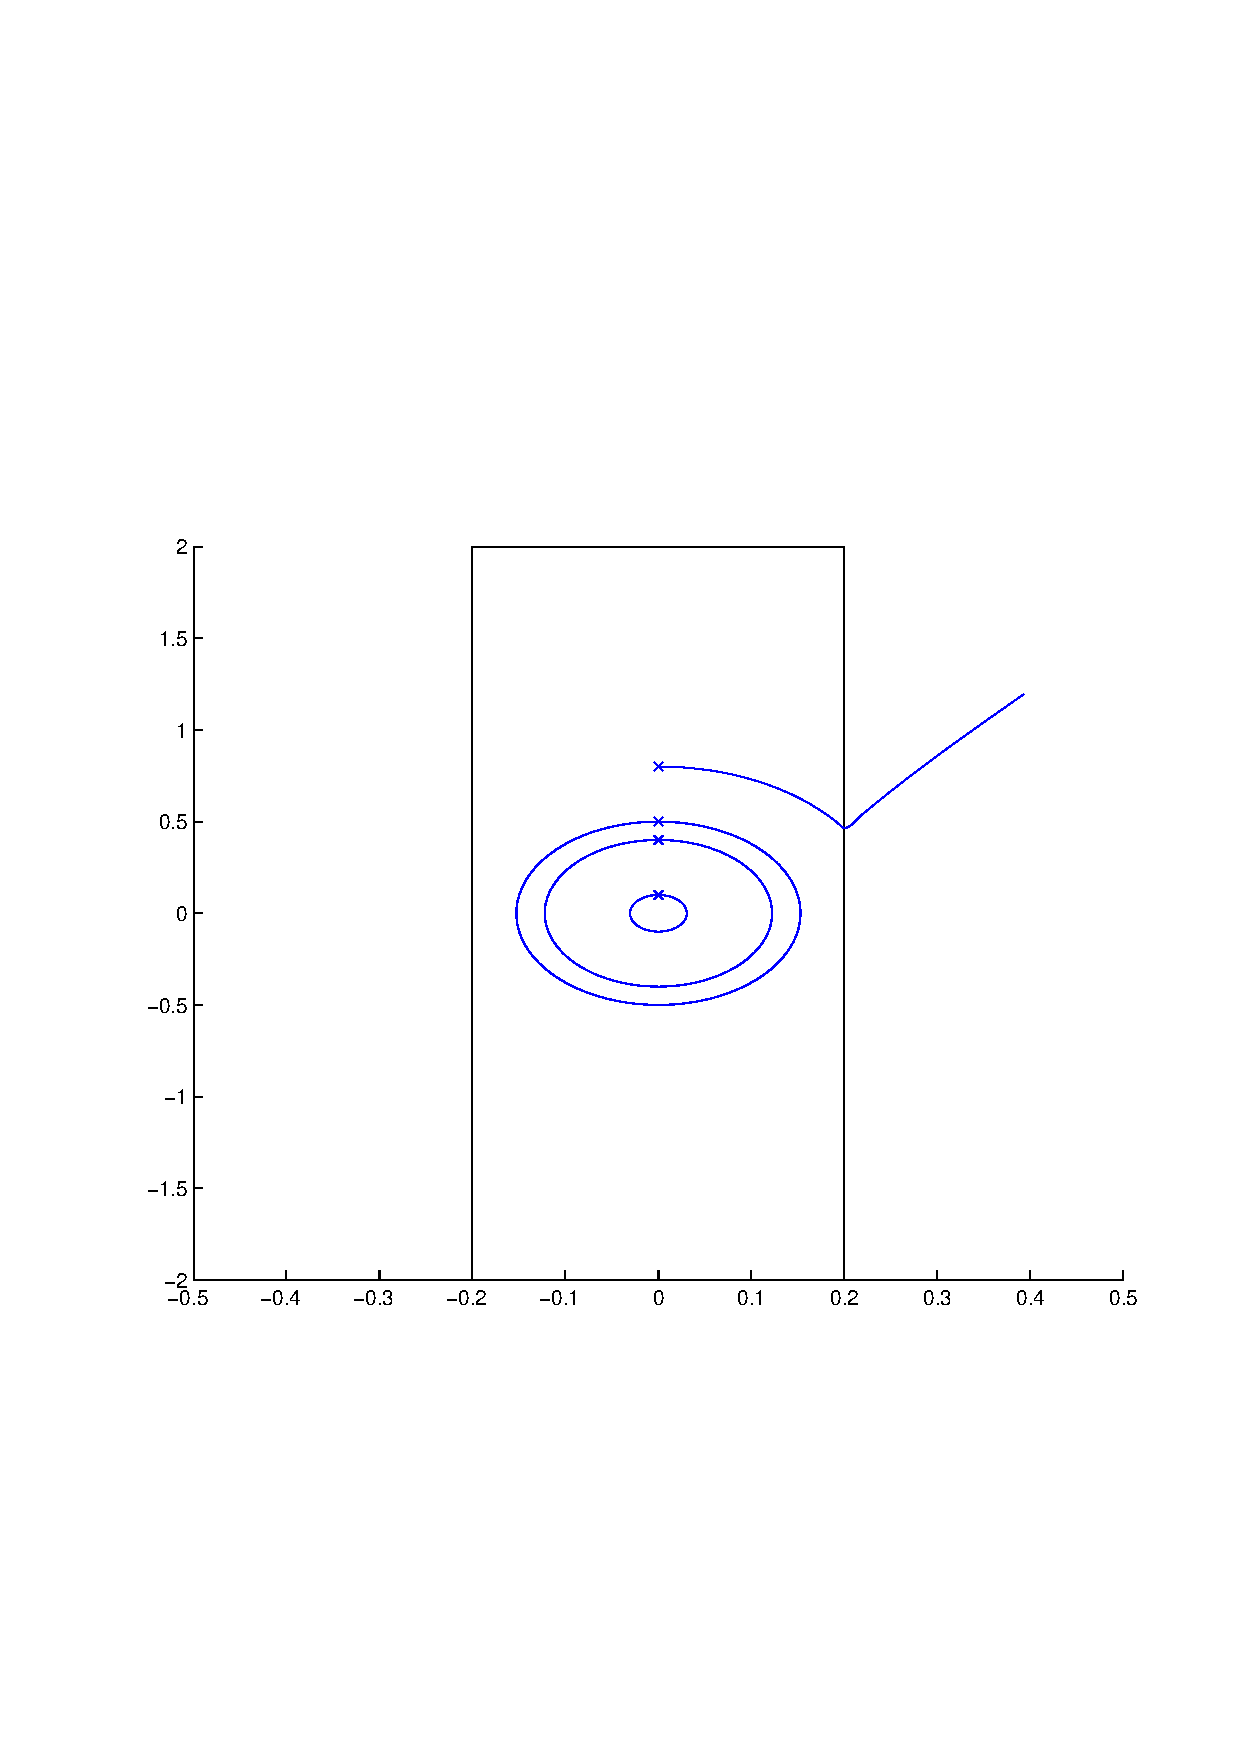
\includegraphics[width=0.7\textwidth]{uncontrolled}
    \caption{un controlled motion}
    \label{fig:stancepostures}
\end{center}
\end{figure}





By coupling neural system the oscillator, the position of the centre is feed into the neural oscillator and the output of neural oscillator drive the torque generated by the legs.
\[
\uin=\hin(q_1)\\
\uout=\tau_{L,R}
\]
Entrainment happens and a limit cycle is formed

but for stance, entrainment does not boost the stability.
it is impossible for mechanical system to converge to the limit circle within $1/4$ period, neural oscillator will not modify the boundary.


\subsection{Local Invariant Control}
All the three group actions can be applied, but two group actions are useful and affects the stability.
\subsubsection*{Time Scaling}
Time scaling action will stretch the phase plot in the velocity direction, as shown in Figure~\ref{fig:stanceTimeScaling}.
It will enlarge the basin of attraction to include high speed state.
\begin{figure}[!htbp]
  \begin{center}
      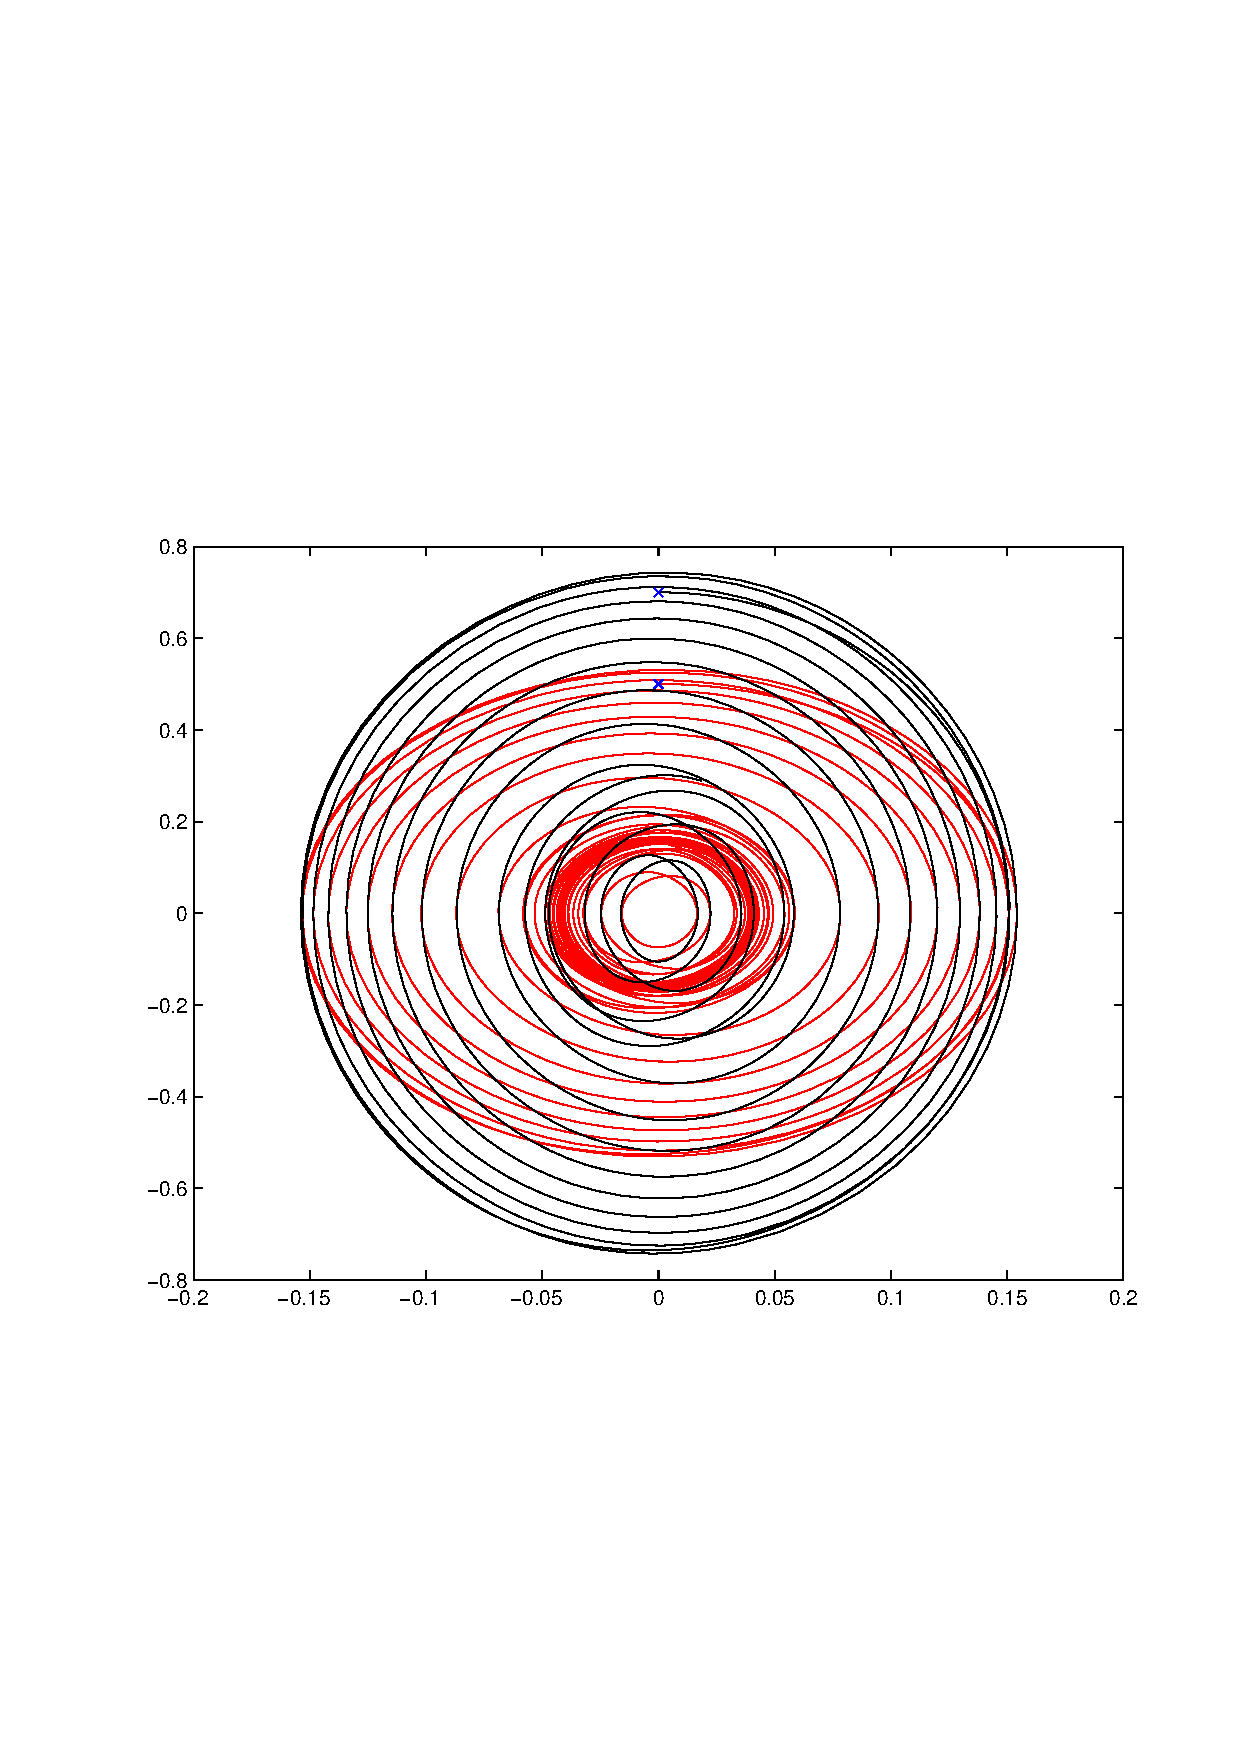
\includegraphics[width=0.7\textwidth]{TimeScaling}
    \caption{Time Scaling}
    \label{fig:stanceTimeScaling}
\end{center}
\end{figure}



\subsubsection*{Energy Control}
By Applying energy scaling action, this will modify the size of the limit cycle,as shown in Figure~\ref{fig:energyscaling}
It will modify the final wobbling amplitude.
but when energy scaling is applied to shrink the limit cycle,
it will also shrink the size of basin of attraction.


\begin{figure}[!htbp]
  \begin{center}
      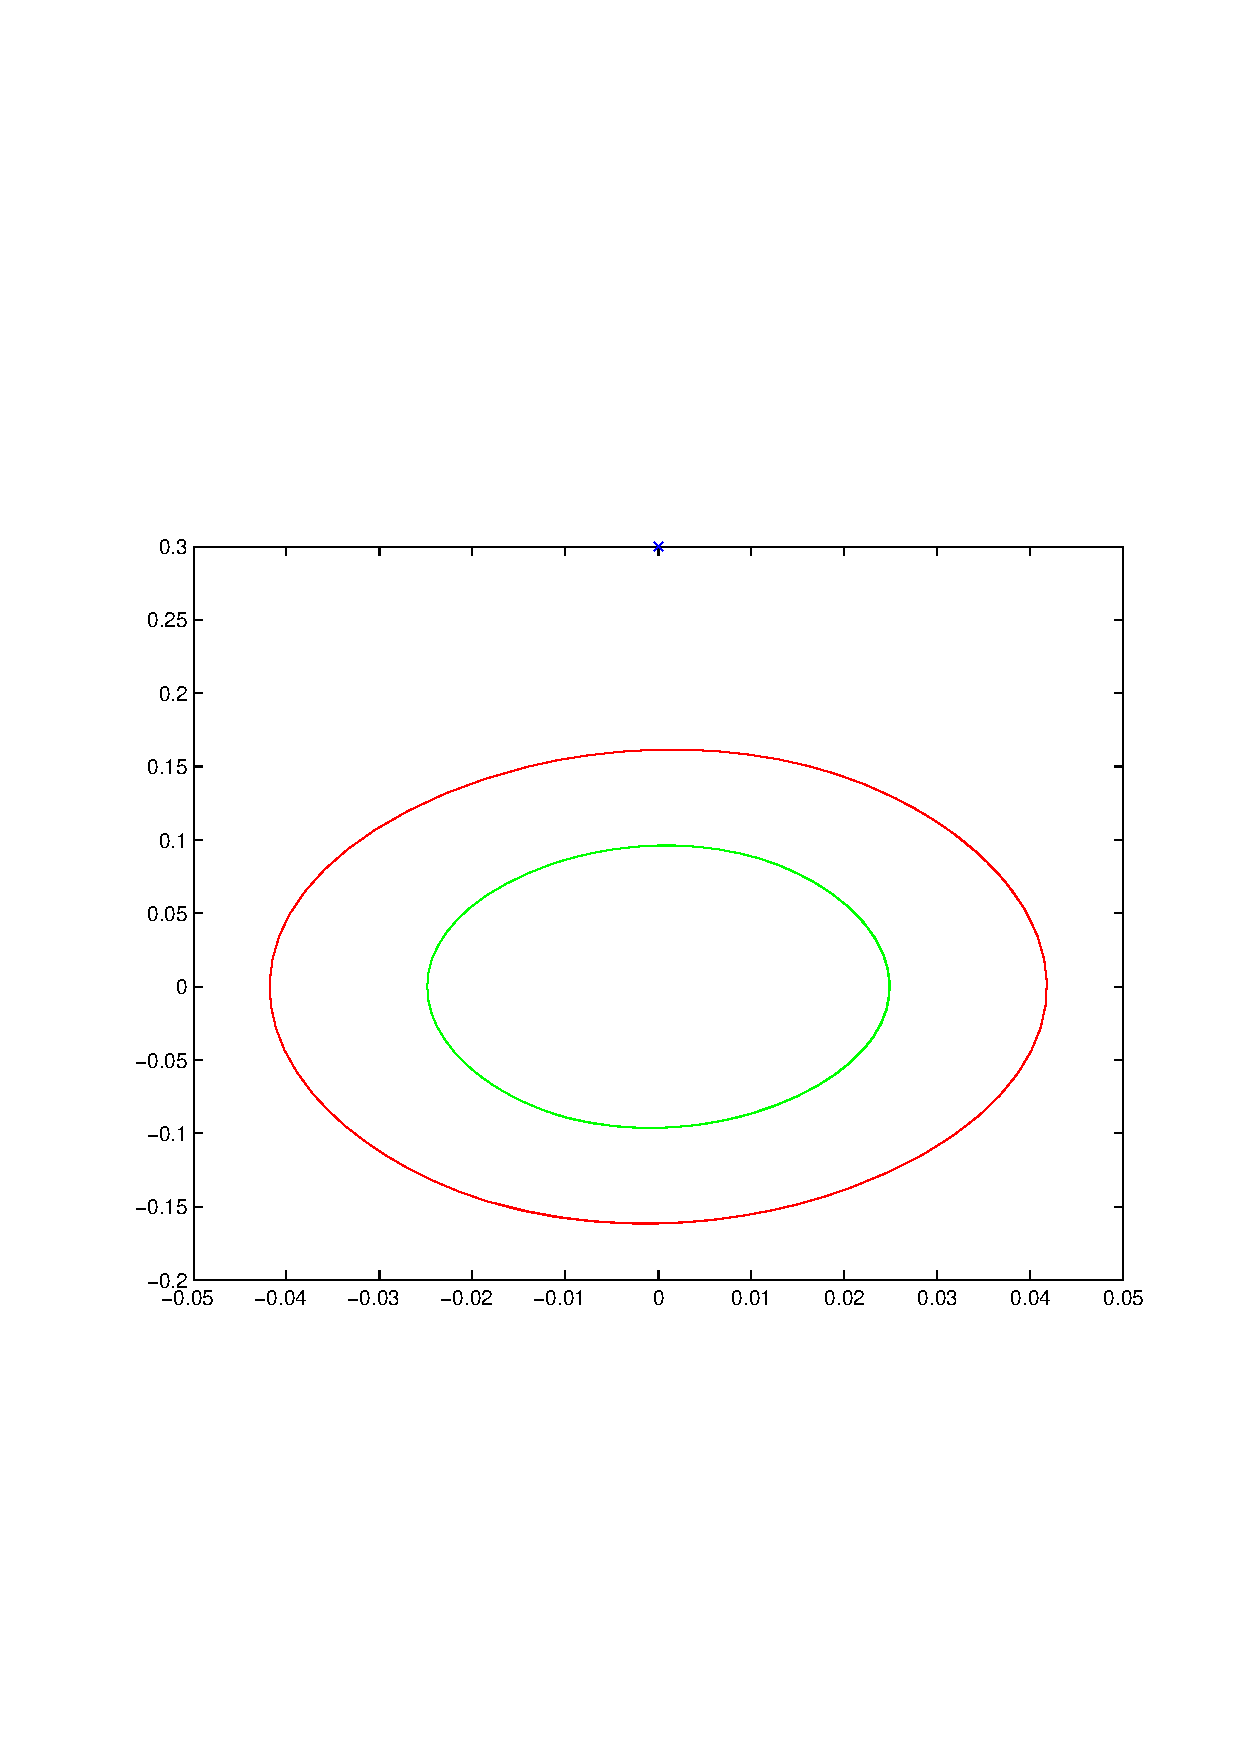
\includegraphics[width=0.7\textwidth]{EnergyControlled}
    \caption{Energy Scaling}
    \label{fig:energyscaling}
\end{center}
\end{figure}





\subsubsection*{Fast Stable}
By applying speed and energy scaling sequencer, wobbling can converge to the limit cycle and stopped quickly.
In Figure ~\ref{fig:fastconverg}, at first speed action is applied to include the high speed state for $1/4$ period, when the state reach the pos that the speed is zero, then energy scaling is applied for $1/4$ period to shrink the limit cycle size.
And for the next $1/4$ period, speed action is applied, and so on.

\begin{figure}[!htbp]
  \begin{center}
      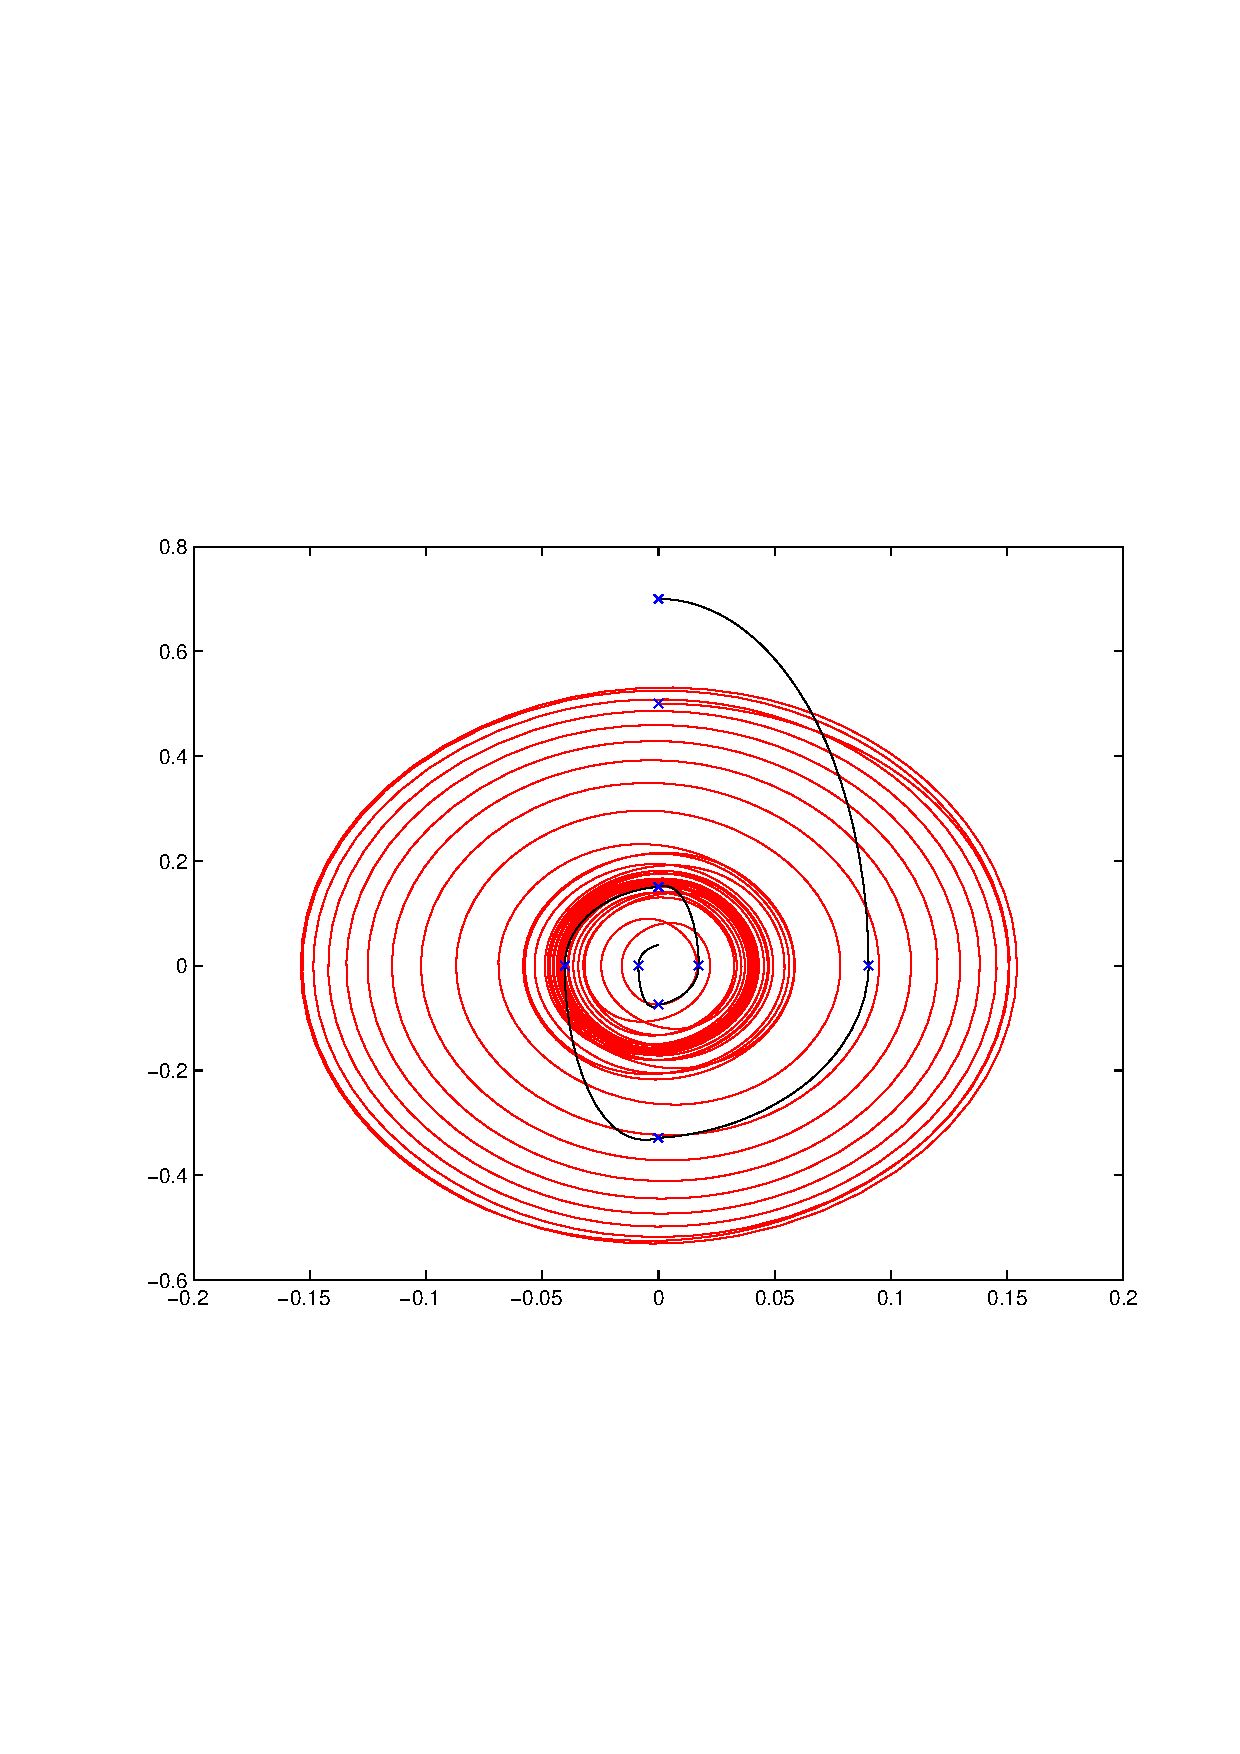
\includegraphics[width=0.7\textwidth]{FastCoverge}
    \caption{Fast Converge}
    \label{fig:fastconverg}
\end{center}
\end{figure}


Motions of stance are put together for comparison.
Without any control and the character fail as shown in Figure~\ref{fig:stancefall}.
In Figure~\ref{fig:stancespeed}, speed action is applied, characters maintain its stance motion, but wobble.
In Figure~\ref{fig:fastconverge}, both speed action and energy action are applied, the character maintain the stance and also vibrate with shrinking amplitude.




\begin{figure}[h]
\begin{center}$
\begin{array}{ccccc}
\includegraphics[width=1in]{stanceFall/0001.eps}&
\includegraphics[width=1in]{stanceFall/0021.eps}&
\includegraphics[width=1in]{stanceFall/0041.eps}&
\includegraphics[width=1in]{stanceFall/0061.eps}&
\includegraphics[width=1in]{stanceFall/0081.eps}
\\
\includegraphics[width=1in]{stanceFall/0101.eps}&
\includegraphics[width=1in]{stanceFall/0121.eps}
\end{array}$
\end{center}
\caption{Balance Motion without Neural Control}
    \label{fig:stancefall}
\end{figure}

\begin{figure}[!htbp]
  \begin{center}
  $
     \begin{array}{ccccc}
\includegraphics[width=1in]{stancewobble/0001.eps}&
\includegraphics[width=1in]{stancewobble/0021.eps}&
\includegraphics[width=1in]{stancewobble/0041.eps}&
\includegraphics[width=1in]{stancewobble/0061.eps}&
\includegraphics[width=1in]{stancewobble/0081.eps}
\\
\includegraphics[width=1in]{stancewobble/0101.eps}&
\includegraphics[width=1in]{stancewobble/0121.eps}&
\includegraphics[width=1in]{stancewobble/0141.eps}&
\includegraphics[width=1in]{stancewobble/0161.eps}&
\includegraphics[width=1in]{stancewobble/0181.eps}

\end{array}$
    \caption{Stance But Wobble}
    \label{fig:stancespeed}
\end{center}
\end{figure}



\begin{figure}[!htbp]
  \begin{center}
        $\begin{array}{ccccc}
\includegraphics[width=1in]{stanceconverge/0001.eps}&
\includegraphics[width=1in]{stanceconverge/0021.eps}&
\includegraphics[width=1in]{stanceconverge/0041.eps}&
\includegraphics[width=1in]{stanceconverge/0061.eps}&
\includegraphics[width=1in]{stanceconverge/0081.eps}
\\
\includegraphics[width=1in]{stanceconverge/0101.eps}&
\includegraphics[width=1in]{stanceconverge/0121.eps}&
\includegraphics[width=1in]{stanceconverge/0141.eps}&
\includegraphics[width=1in]{stanceconverge/0161.eps}&
\includegraphics[width=1in]{stanceconverge/0181.eps}

\end{array}$
    \caption{Stance And Stable}
    \label{fig:fastconverge}
\end{center}
\end{figure}




\section{Walking and Stance Transition}
Both limit cycles of walking and stancing are shown in Figure~\ref{fig:walksstance}.
the phase plot here shows the supporting leg, the swing leg is show in shadow red






\subsection{Walk to Stance}
walk to stance transition happens at the heel strike phase.
if without control effort, the bipedal machine will continue two walk, while if we switch the on the stance controller,
the bipedal machine will converge to a small amplitude,then both legs start oscillation, this is the stance to walk.

\begin{figure}[!htbp]
  \begin{center}
    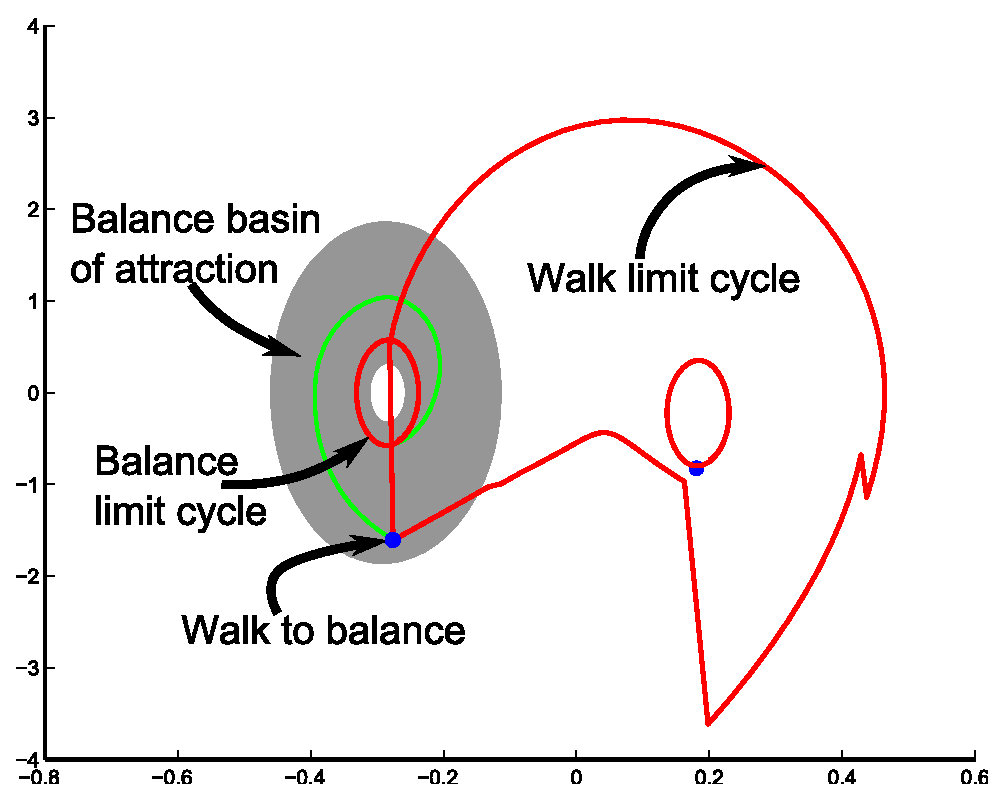
\includegraphics[width=0.7\textwidth]{walk_to_stand}
    \caption{Fast Converge}
    \label{fig:walksstance}
	\end{center}
\end{figure}



%\begin{figure}[!htbp]
%  \begin{center}
%      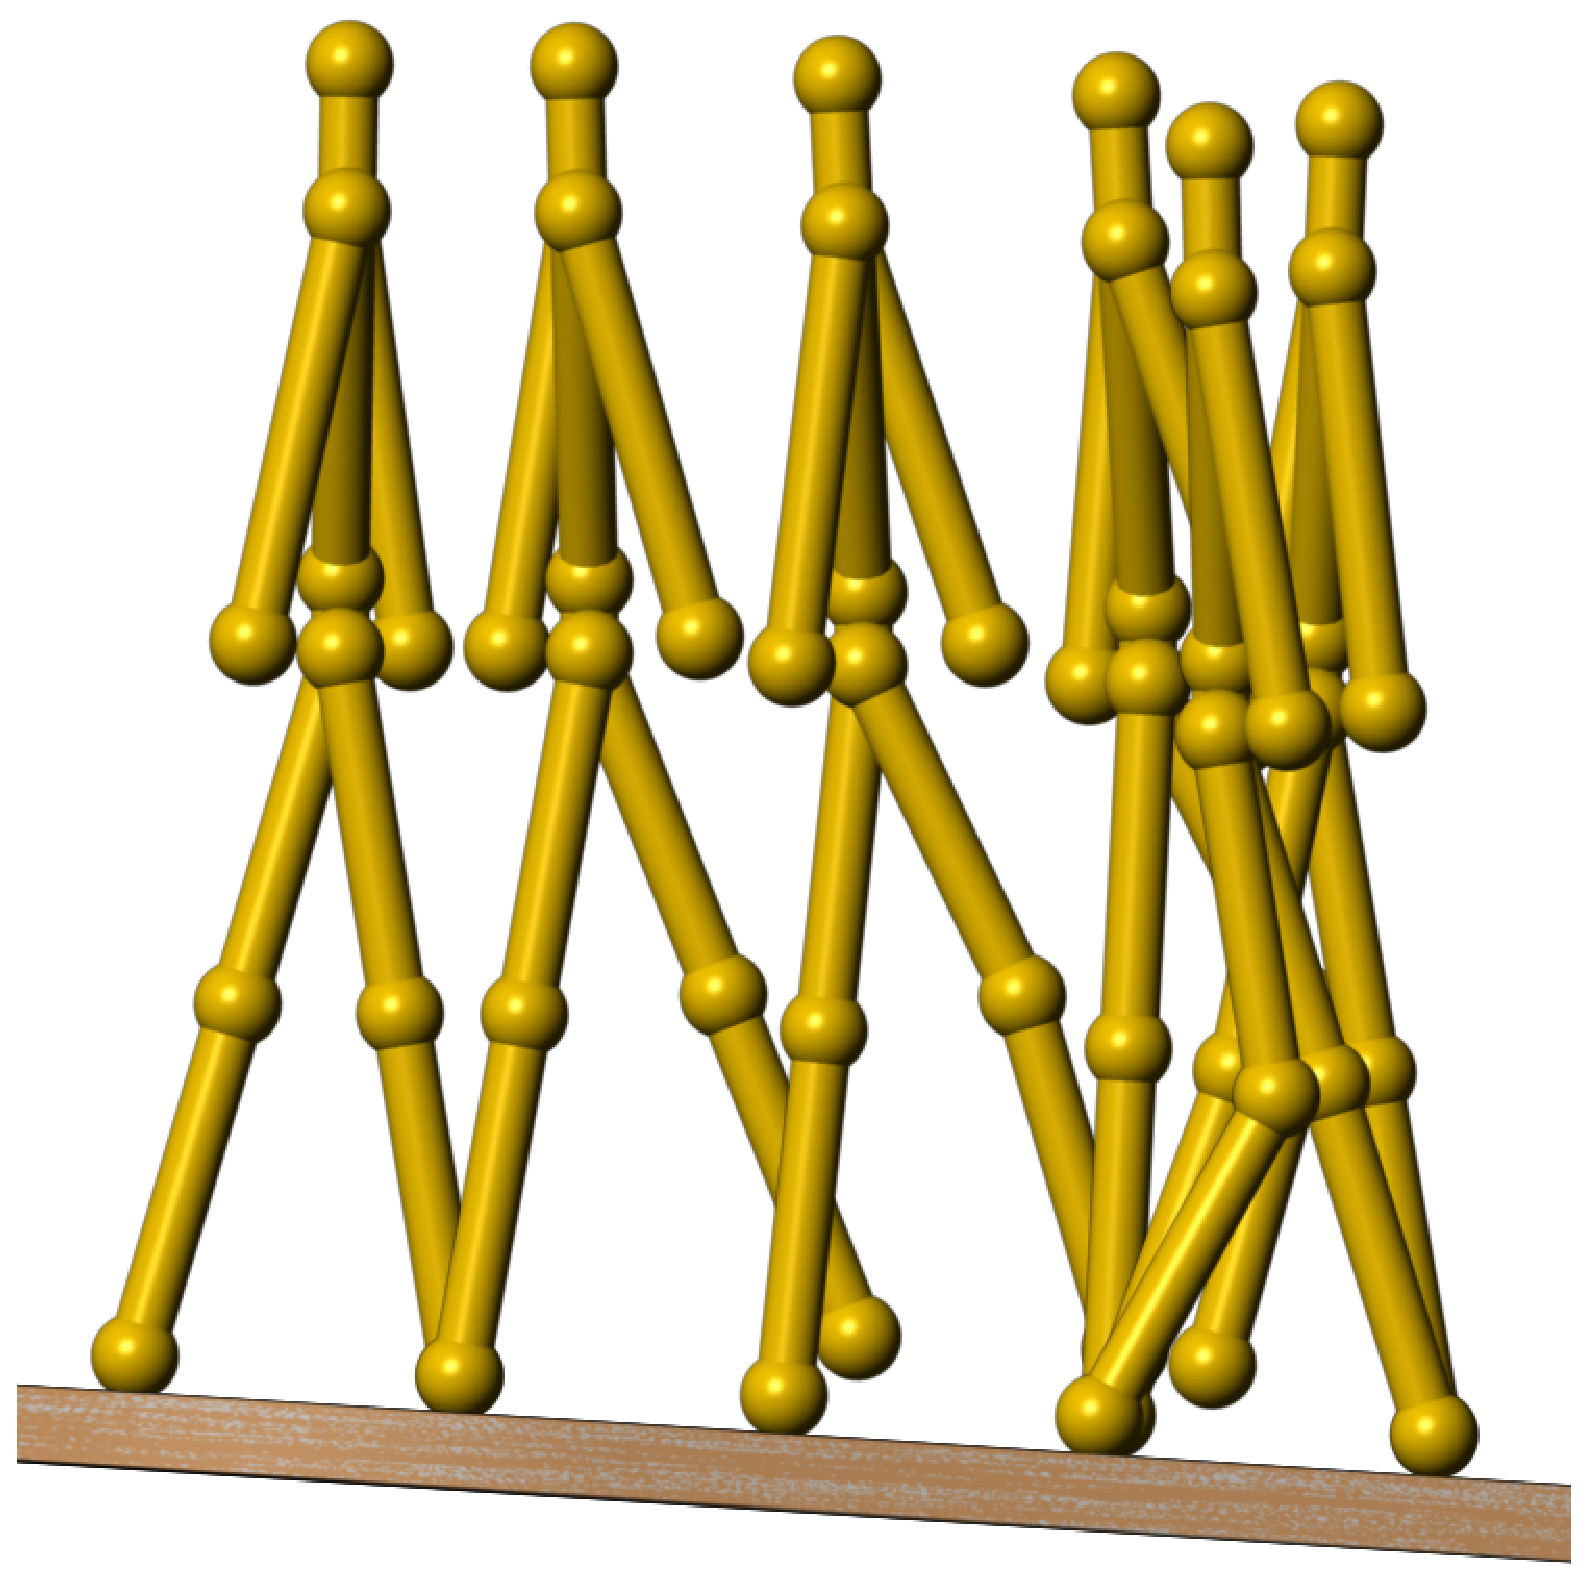
\includegraphics[width=0.7\textwidth]{walk_to_balance}
%    \caption{Walk to Balance}
%    \label{fig:walk2stance}
%\end{center}
%\end{figure}




\subsubsection*{Knee Bending Scheme}
During walk to stance transition, when the heel strikes, the two legs are straight. 
At this time, the support region is very small.
Any push of the figure, it will move out of the two support region.
To enlarge the basin of attraction, the walkers have to bend legs and lower the height.
Many possible ways can be develop for bending the legs.


\begin{itemize}
	\HiItem{One Leg Bending}
		walker can bend one leg while keep the other leg straight.
	\HiItem{Double Leg Bending}
		We can make the two leg bend.
\end{itemize}

It is very difficult to tell which one more realistic for when human walk, the knees is not necessary straight.
Motion of Double Leg Bending  are shown in Figure~\ref{fig:walkstancestraight}.

\begin{figure}[!htbp]
  \begin{center}
        $\begin{array}{ccccc}
\includegraphics[width=1in]{WalkStanceTransition/0001.eps}&
\includegraphics[width=1in]{WalkStanceTransition/0101.eps}&
\includegraphics[width=1in]{WalkStanceTransition/0201.eps}&
\includegraphics[width=1in]{WalkStanceTransition/0301.eps}&
\includegraphics[width=1in]{WalkStanceTransition/0401.eps}
\\
\includegraphics[width=1in]{WalkStanceTransition/0501.eps}&
\includegraphics[width=1in]{WalkStanceTransition/0601.eps}&
\includegraphics[width=1in]{WalkStanceTransition/0701.eps}&
\includegraphics[width=1in]{WalkStanceTransition/0801.eps}&
\includegraphics[width=1in]{WalkStanceTransition/0901.eps}
\end{array}$
      
    \caption{Stop Walking with Two Leg Bend}
    \label{fig:walkstancestraight}
\end{center}
\end{figure}



\subsection{Stance to Walk}
For walk stance transition, we must move the state close to the walking limit cycle.
we should place the state of the near the position of start swing position (show in blue).
On the limit cycle of stance, this is the position that the leg is moving forward at maxim speed and the position of the hip is in the middle between the two legs.
if we switch to the walker at this time, then it will begin to walk.



From stance to walk, there the height has to be increase, so there are only one scheme for straight the knees.
the scheme we use is to keep the front leg straight and make the hind leg from bend to straight.
as show in Figure~\ref{fig:stance2walk}.
\begin{figure}[!htbp]
  \begin{center}
     \includegraphics{stance2walk}
    \caption{The Phase Plot for Stance to Walk}
    \label{fig:stance2walk}
\end{center}
\end{figure}


A non-trivial problem is when switch from stance to walk, 
It is impossible to put both legs on the limit cycle
The supporting leg is been given the priority, for the support leg is more important for maintaining stability.





\subsection{Speed Action Connection}
When transit from walk to stance, the basin of attraction must include the heel strike state.
original basin of attraction will not include the heel strike; a speed action is needed to enlarge the basin of attraction.
There is an alternative to this, we can lower the walker speed, in this way, and we lower the action of balance control.

Also, if transition from stance to walk, if little effort is executed, the it will start at pos far from the limit cycle.
then to maintain the stability walking, speed action needed to include for start walking slowing.

So the speed action of stanching and walking must meet some relationship as
The phenomenon is common for our daily experience; here we give it a mathematical meaning.
\[
\frac{S_s}{S_w}=c
\]

























